%Matteo Kumar - Leonard Schatt
% Fortgeschrittenes Physikalisches Praktikum
% Main-Datei für die Auswertung in TeX

% Struktur:
% Für jeden Abschnitt gibt es einen Ordner, damit jeder individuell an seinen Aufgaben arbeiten
% kann, ohne beim merge in GitHub Konflikte zu erhalten. Deshalb werden alle Unteraufgaben auch 
% extra in Ordner angelegt. Die einzelnen Dateien über den input Befehl einfügbar.
% Bilder und andere Grafik werden im Ordner Grafik abgelegt 


% Packages
\documentclass[paper=a4,bibliography=totoc,BCOR=10mm,twoside,numbers=noenddot,fontsize=11pt]{scrreprt}
\usepackage[ngerman]{babel}
\usepackage[latin1, utf8]{inputenc}
\usepackage[babel,german=quotes]{csquotes} %For Quotes
\usepackage[T1]{fontenc}
\usepackage{lmodern}
\usepackage{graphicx}
\usepackage{nicefrac}
\usepackage{fancyvrb}
\usepackage{amsmath,amssymb,amstext}
\usepackage{siunitx}
\usepackage{url}
\usepackage{natbib}
\usepackage{microtype}
\usepackage[format=plain]{caption}
\usepackage{physics}
\usepackage{titleref}

% Zusätzliche Packages
\usepackage{geometry}
\usepackage{anyfontsize}
\usepackage[table]{xcolor}
\usepackage{ifthen}
\usepackage[absolute,overlay]{textpos}
\usepackage{amsfonts}
\usepackage{xstring}
\usepackage{tikz}
\usepackage{pdfpages}
\usepackage{booktabs}
\usepackage{hyperref}

% Abschnittseinrückung und -abstand
% Die folgenden Zeilen sollen möglichst nicht verändert werden
\parindent 0.0cm
\parskip 0.8ex plus 0.5ex minus 0.5ex

% Anzahl und Größe von Gleitobjekten
% maximal 2 Objekte oben und unten
% erlaubt auch größere Bilder, welche die ganze Seite benötigen
% Die folgenden Zeilen sollen möglichst nicht verändert werden
\setcounter{bottomnumber}{2}
\setcounter{topnumber}{2}
\renewcommand{\bottomfraction}{1.}
\renewcommand{\topfraction}{1.}
\renewcommand{\textfraction}{0.}

%\sc und \bc veraltet. Daher: (20.09.2018)
\DeclareOldFontCommand{\sc}{\normalfont\scshape}{\@nomath\sc}
\DeclareOldFontCommand{\bf}{\normalfont\scshape}{\textbf}

% Verschiedenes
\pagestyle{headings}          % Der Seitenstil sollte möglichst nicht verändert werden
\graphicspath{{./bilder/}}    % Der Pfad für die Abbildungen Abbildungen wird gesetzt
\VerbatimFootnotes            % \verb etc.

% Funktionen
\newcommand\tab[1][1cm]{\hspace*{#1}}
\newcommand{\vect}[1]{\boldsymbol{\mathbf{#1}}}
\newcolumntype{g}{>{\columncolor[rgb]{ .741,  .843,  .933}}l}
% Tiefgestellte Zahlen nicht kursiv
\catcode`_=\active
\newcommand_[1]{\ensuremath{\sb{\mathrm{#1}}}}

\begin{document}

    \nonfrenchspacing

    % 0. Kapitel 
    % Manuel Lippert - Paul Schwanitz
% Physikalisches Praktikum

% 0. Cover
% Noch abänderbar nur ein Vorschlag
\newgeometry{top=30mm, bottom=20mm, inner=20mm, outer=20mm}
\thispagestyle{empty}

% Colors
\definecolor{Notablue}{HTML}{3498DB}		%Theoretische Physik
\definecolor{Notared}{HTML}{CF366C}			%Mathematik
\definecolor{Notagreen}{HTML}{19B092}		%Experimentalphysik
\definecolor{Notaorange}{HTML}{FA9D00}		%Chemie/Wahlfach nicht physikalisch
\definecolor{Notagrey}{HTML}{969696}		%Praktikum
\definecolor{Notalavendel}{HTML}{9DBBD8}	%Wahlfächer physikalisch

% Boolean by default false
\newboolean{twoRows}
\newboolean{symbol}

% Funktions
\makeatletter
   \def\vhrulefill#1{\leavevmode\leaders\hrule\@height#1\hfill \kern\z@}
\makeatother
\newcommand*\ruleline[1]{\par\noindent\raisebox{.8ex}{\makebox[\linewidth]{\vhrulefill{\linethickness}\hspace{1ex}\raisebox{-.8ex}{#1}\hspace{1ex}\vhrulefill{\linethickness}}}}

% Variables
\def\schriftgrosse{40}
\def\linethickness{1,5pt}

\def\farbe{black}
\def\fach{PPBphys2}
\def\name{Manuel Lippert - Paul Schwanitz}
\def\uberschrift{Chaos in einfachen \\[0,5cm] physikalischen Systemen} % Absatz mit \\[0,5cm]; u = Übung, k = Klausur; s = Skript, e = Ergebnis
\def\bottom{WS2021/22}
\def\datum{06.09.2021}
\def\platz{B11 | 0.09}
\def\betreuer{Reinhard Richter}

\def\teilnehmerm{Manuel Lippert}
\def\emailm{Manuel.Lippert@uni-bayreuth.de}
\def\teilnehmerp{Paul Schwanitz}
\def\emailp{Paul.Schwanitz@uni-bayreuth.de}

%\def\auswertp{}
%\def\messp{}
%\def\protop{}

\def\groupnr{11}

\begin{titlepage}
			
	\centering
	{\LARGE \sffamily {\textbf{\bottom}\par}}
	\vspace{2,5cm}
    {\fontsize{30}{0}\sffamily\ruleline{\textcolor{\farbe}{\textbf{\fach}}}\par}
    \vspace{6cm}
	{\Large\sffamily \ruleline{\name}\par}
	
	
	% Choose Text
	\ifthenelse{\equal{\uberschrift}{s}} {\def\titel{Skript}}	
		{\ifthenelse{\equal{\uberschrift}{k}} {\def\titel{Klausur}}
			{\ifthenelse{\equal{\uberschrift}{u}} {\def\titel{Übung}}
				{\ifthenelse{\equal{\uberschrift}{e}} {\def\titel{Klausur \\[0,5cm] Ergebnis}}
					{\def\titel{\uberschrift}}
				}
			}
		}
	
	\IfSubStr {\titel} {\\[0,5cm]} {\setboolean{twoRows}{true}} {\setboolean{twoRows}{false}}
	
	\ifthenelse{\boolean{twoRows}}
		{
			\begin{textblock*}{21cm}(0cm,8,5cm) % {block width} (coords), centered		
				{\fontsize{\schriftgrosse}{0}\sffamily\textcolor{\farbe}{\textbf{\titel}}\par}
			\end{textblock*}
		}
		{
			\begin{textblock*}{21cm}(0cm,9cm) % {block width} (coords), centered		
				{\fontsize{\schriftgrosse}{0}\sffamily\textcolor{\farbe}{\textbf{\titel}}\par}
			\end{textblock*} 
		}
	
	% Choose Logo
	\ifthenelse {\equal{\farbe}{Notared}} {\def\logo{Bilder/Logo/UniBTNotared}}
		{\ifthenelse {\equal{\farbe}{Notagreen}} {\def\logo{Bilder/Logo/UniBTNotagreen}}
			{\ifthenelse {\equal{\farbe}{Notablue}} {\def\logo{Bilder/Logo/UniBTNotablue}}
				{\ifthenelse {\equal{\farbe}{Notaorange}} {\def\logo{Bilder/Logo/UniBTNotaorange}}
					{\ifthenelse {\equal{\farbe}{Notagrey}} {\def\logo{Bilder/Logo/UniBTNotagrey}}
						{\ifthenelse {\equal{\farbe}{Notalavendel}} {\def\logo{Bilder/Logo/UniBTNotalavendel}}	
							{\ifthenelse {\equal{\farbe}{black}} {\def\logo{Bilder/Logo/UniBT}}	
								{\def\logo{noLogo}}
							}
						}
					}
				}
			}
		}	

	\IfSubStr{\logo}{noLogo}{\setboolean{symbol}{false}}{\setboolean{symbol}{true}}
	
	% Gruppe
	\vspace{10cm}
	{\large\sffamily{Gruppe \groupnr}}
	
	%Logo
	\vfill

	\ifthenelse{\boolean{symbol}}
		{
			\begin{figure}[h]
			\begin{center}
				
				\includegraphics[width=2cm]{\logo}
				
			\end{center}
			\end{figure}
		}
	
\end{titlepage}

\restoregeometry

% Information
\chapter*{Informationen}
\label{chap:info}

\begin{tabular}{l l}

	{\textbf{Versuchstag}} \hspace{1cm} & \hspace{1cm} {\datum}\\[0,2cm]
	{\textbf{Versuchsplatz}} \hspace{1cm} & \hspace{1cm} {\platz}\\[0,2cm]
	{\textbf{Betreuer}} \hspace{1cm} & \hspace{1cm} {\betreuer}\\[1,2cm]
	{\textbf{Gruppen Nr.}} \hspace{1cm} & \hspace{1cm} {\groupnr}\\[0.2cm]
	{\textbf{Teilnehmer}} \hspace{1cm} & \hspace{1cm} {\teilnehmerm}\\[0.2cm]
						  \hspace{1cm} & \hspace{1cm} {\emailm}\\[0.2cm]
						  \hspace{1cm} & \hspace{1cm} {\teilnehmerp}\\[0.2cm]
						  \hspace{1cm} & \hspace{1cm} {\emailp}\\[0.2cm]

	%{\textbf{Auswertperson}} \hspace{1cm} & \hspace{1cm} {\auswertp}\\[0.2cm]
	%{\textbf{Messperson}} \hspace{1cm} & \hspace{1cm} {\messp}\\[0.2cm]
	%{\textbf{Protokollperson}} \hspace{1cm} & \hspace{1cm} {\protop}\\[0.2cm]

\end{tabular}

    \thispagestyle{empty}
    \cleardoublepage
    \tableofcontents
    \cleardoublepage

    % 1. Kapitel Einleitung
    %Matteo Kumar - Leonard Schatt
% Fortgeschrittenes Physikalisches Praktikum

% 1. Kapitel Einleitung

\chapter{Einleitung}
\label{chap:einleitung}

Radioaktivität ist ein uns immer umgebender Umweltfaktor. Dabei ist sie - neben den gesundheitlichen Schäden, die sie verursachen 
kann - oft ein nützliches Hilfsmittel. Sie kann zu medizinischen Zwecken eingesetzt werden, oder zur Materialanalyse. 
Dabei sind vor allem Alpha- und Gammastrahlung für die Identifikation von Materialien wichtig. Da diese diskrete und charakteristische 
Spektren haben, kann man mit diesen bestimmte radioaktive Isotope nachweisen. Dies werden wir in diesem Versuch durchführen. Des Weiteren 
verwenden wir die Strahlung zur Schichtdickenmessung. Insgesamt erhöht der Versuch die Kompetenzen im Umgang mit radioaktiven Präparaten und 
macht sensibler für die damit verbundenen Gefahren.


    % 2.Kapitel Fragen zur Vorbereitung
    %Matteo Kumar - Leonard Schatt
% Fortgeschrittenes Physikalisches Praktikum
 

% Matteo Kumar
% PPB2 AFM
%Grundlagen

\chapter{Grundlagen}

\section{FRET}

Förster-Resonanzenergietransfer ist ein Prozess des Energietransfers. Dabei gibt es einen Donor und einen Akzeptor. Der Donor gibt dabei über Dipol-Dipol-Wechselwirkung 
Energie an den Akzeptor ab – und das strahlungsfrei.
Damit FRET auftritt müssen bestimmte Voraussetzungen erfüllt sein. Zunächst müssen sich das Emissionsspektrum des Donors und das Absorptionsspektrum des Akzeptors überlappen wie in  
Abbildung \ref{bild:FRETSpektrum} zu sehen.

\begin{figure}[h]
    \centering
    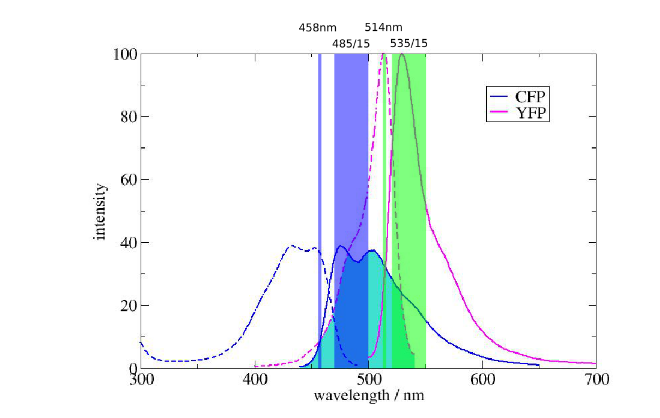
\includegraphics[width = 10cm]{Bilder/Grundlagen/FRETSpektrum.png}
    \caption{Emissionsspektrum/Absorptionsspektrum von CPF/YFP (\cite{FRETSkript})}
    \label{bild:FRETSpektrum}
\end{figure}

Sollte dies der Fall und der Abstand zwischen Akzeptor und Donor klein genug sein, dann tritt FRET auf. \\
Der Abstand muss klein genug sein, da die FRET-Effizienz\\


\begin{equation}
    E = \frac{1}{1+\frac{r^6}{R_0^6}}
\end{equation}

ist. Dabei bezeichnet $R_0$ den Försterradius und $r$ den Abstand der beiden Moleküle. Man sieht seht schön, dass $E = 1/2$ ist für $r = R_0$. Das ist auch die 
Definition des Försterradiuses: Die Hälfte der einfallenden Photonen, die vom Donor absorbiert werden, werden über FRET auf den Akzeptor übertragen.\\
Der Försterradius liegt normalerweise im Nanometerbereich, da die Dipol-Dipol-Wechselwirkung sehr kurzreichweitig ist. Daher kommt auch die sechste Potenz unter dem Bruchstrich.\\
Wichig ist noch, dass ein Teil der Energie als Vibration bei dem emittierenden Molekül bleibt. Daher ist die emittierte Strahlungen energieärmer als die absorbierte Strahlungen. Außerdem 
ist der Prozess stark orientierungsabhängig, da Dipole dies auch sind.


\section{Photobleichung}

Die Photobleichung ist ein Prozess, bei dem die Fluoreszenzeigenschaften einen Fluorophors vollständig verloren gehen. 
Dies geschieht, indem man das Fluorophor mehrfach anregt. Ein Fluorophor hat eine durchschnittliche Anzahl an Anregungs- und Emissionszyklen. 
Bei zu häufiger Anregung wir das Fluorophor inaktiviert, indem es im Molekül zu einer photochemischen 
Reaktion kommt. Dabei kann ein Elektron, was auf eine höhere Schale gehoben wurde, zu irreversibel kovalenten Änderung am 
Fluorophor führen (\cite{Song1995}).

\section{Konfokalmikroskop}

Ein Konfokalmikroskop (siehe Abb. \ref{bild:Konfokalmikroskop}) ist ein Mikroskop, was im Gegensatz zum klassischen Mikroskop nicht die gesamte Probe beleuchtet. 
Stattdessen beleuchtet es Punktweise die Probe mit einem Laserstrahl. Danach detektiert man die zurückfallende Strahlung, 
beispielsweise bei Fluorophoren die Fluoreszenz. Diese wird durch eine Lochblende geführt, sodass bei kleiner 
Blendenöffnung nur Punkte in einer bestimmten Ebene angezeigt werden. Bei größerer Blende ist die Lichtstärke höher, die betrachtete Ebene ist aber auch tiefer. 

\begin{figure}[ht]
    \centering
    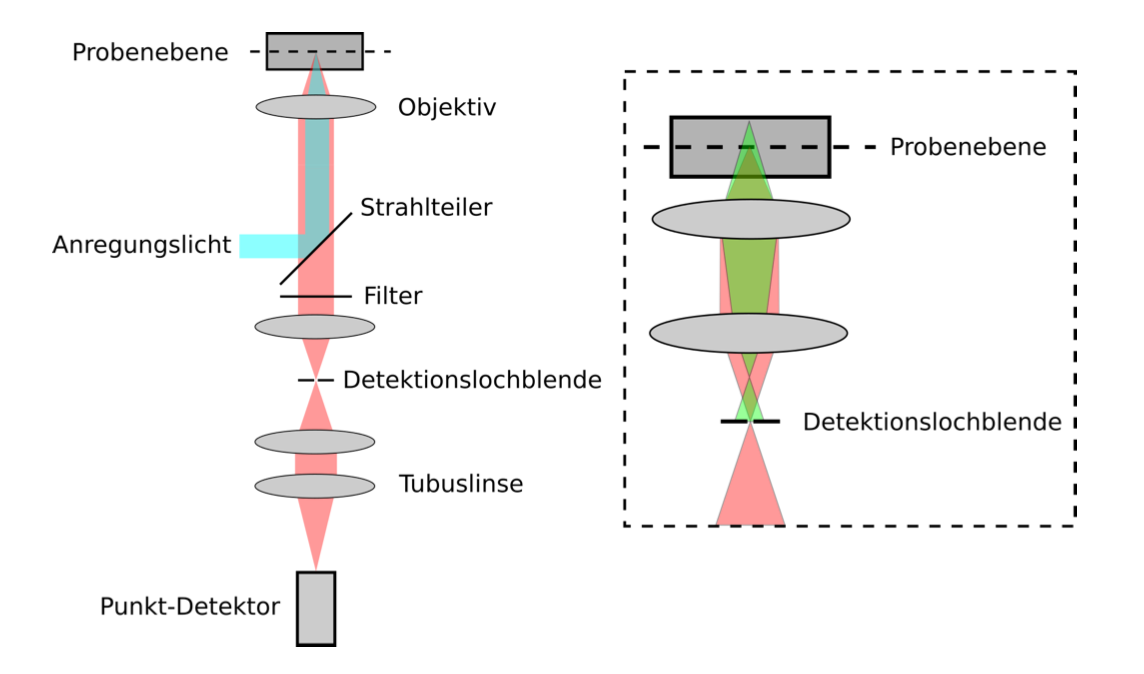
\includegraphics[width = 10cm]{Bilder/Grundlagen/Konfokalmikroskop.png}
    \caption{Skizze eines Konfokalmikroskops und Prinzip der selektiven Detektion (\cite{FRETSkript})}
    \label{bild:Konfokalmikroskop}
\end{figure}

Bei diesem Mikroskop entsteht also zu keinem Zeitpunkt ein vollständiges Bild. Es eignet sich besonders zum untersuchen biologischer Proben. 
Dabei versetzt man diese mit einem fluoreszenten Protein, welches den entsprechden Arealen anhaftet, und mikroskopiert dieses dann. Dadurch kann man 
deutlich kontrastreichere Bilder aufnehmen und beispielsweise Membrane sichtbar machen. 
% Leonhard Schatt

\section{Lock-in Verstärker}

Der Lock-in Verstärker ist ein wichtiges Messgerät. Er wird dazu verwendet schache Signale, die normalerweise weit unter dem Rauschen liegen noch aufzulösen.
Dabei detektiert das Eingangssignal phasenempfindlich. Beim Messen eines Gleichspannungssignals wir das Signal von einem Chopper in den rauscharmen Bereich "hochgemischt". 
Dies geschieht, da bei niedrigen Frequenzen das "rosa Rauschen" dominiert. (\cite{Herink2021}) 

\begin{figure}[h]
    \centering
    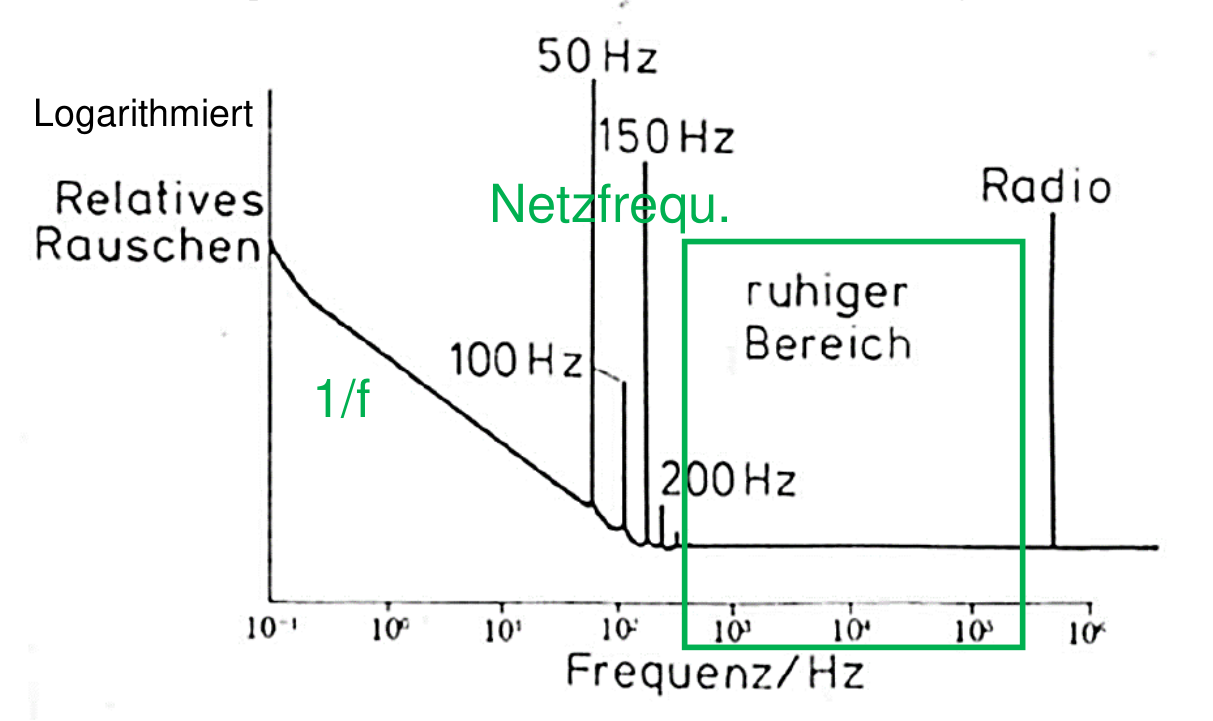
\includegraphics[width = 10cm ]{Bilder/Rauschen.png}
    \caption{Spektrum der Rauschleistung in Abhängigkeit der Frequnez \protect \footnotemark}
\end{figure}
\footnotetext{\cite{Herink2021}}
Im Lock-in Verstärker selbst wird das Signal dann verstärkt und mit einem Referenzsignal $V_R$ gleich der Chopperfrequenz gemischt. Dabei entsteht nach Additiontheoremen für Sinus und Cosinus eine
Differenz- und Summenfrequenz. Dann Filtert man die Differenzfrequenz heraus, indem man einen Tiefpassfilter hinter den Mischer stellt. Im Anschluss wir dann die Spannung abgegriffen. 
Der Vorteil dieses Aufbaus ist, dass die beiden Modulationen durch Chopper und Mischer zusammen wie ein sehr schmalbandiger Filter wirken. Dabei können Bandbreiten von bis zu 0,01Hz erreicht werden. 
Außerdem mittelt sich das Rauschen weg, das es in Beziehung zu $V_R$ unkorreliert ist. Die ausgegebene Spannung hängt jetzt aber noch von der Phasenbeziehung zwischen dem 
modulierten Eingangssignal $V_S$ und dem Referenzsignal $V_R$, das am Mischer ankommt, ab.
\begin{figure}[ht]
    \centering
    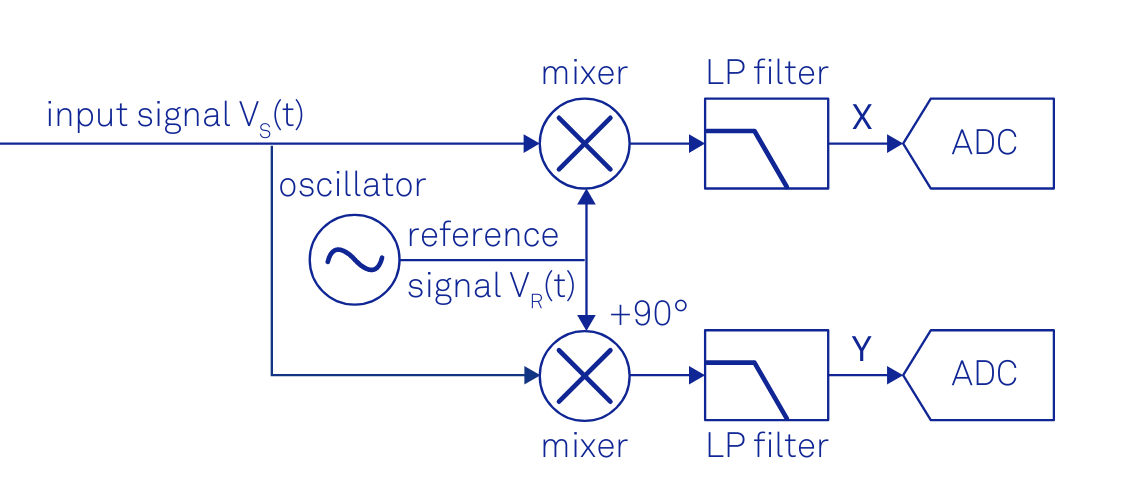
\includegraphics[width = 12cm]{Bilder/Lockin.png}
    \caption{Lock-in Verstärker mit schon moduliertem Eingangssignal $V_S$ \protect \footnotemark}
    \label{lockin}
\end{figure}
\footnotetext{\url{https://www.zhinst.com/sites/default/files/li_primer/zi_whitepaper_principles_of_lock-in_detection.pdf}}
 Deswegen fügt man, wie in Grafik \ref{lockin} zu sehen, einen zweiten Arm ein, on welchen $V_R$ 
um 90° verzögert wird. Aus den beiden Amplituden $X$ und $Y$ berechnet man dann die Amplitude $R$ des Ausgangssignals folgendermaßen:
\begin{equation*}
    R = \sqrt{X^{2}+Y^{2}}
\end{equation*}
  



    % 3.Kapitel Protokoll
    %% Charlotte Geiger - Manuel Lippert - Leonard Schatt
% Physikalisches Praktikum

% 3.Kapitel  Protokoll

% Variables
\def\skalierung{0.65}

\chapter{Messprotokoll}
\label{chap:protokoll}

Das Messprotokoll wurde am Versuchstag handschriftlich erstellt und hier als
PDF-Datei eingefügt. 

\section*{Zusatz}
Zusätzlich fügen wir die Bilder und die verwendeten Schaltungen des Versuchs nch dem Protokoll an zur besseren Übersicht.

% Einbindung des Protokolls als pdf (mit Seitenzahl etc.)
% Erste Seite mit Überschrift
%\includepdf[pages = 1, landscape = false, nup = 1x1, scale = \skalierung , pagecommand={\thispagestyle{empty}\chapter{Protokoll}}]
%            {03-Protokoll/Protokoll.pdf}
% Restliche Seiten richtig skaliert
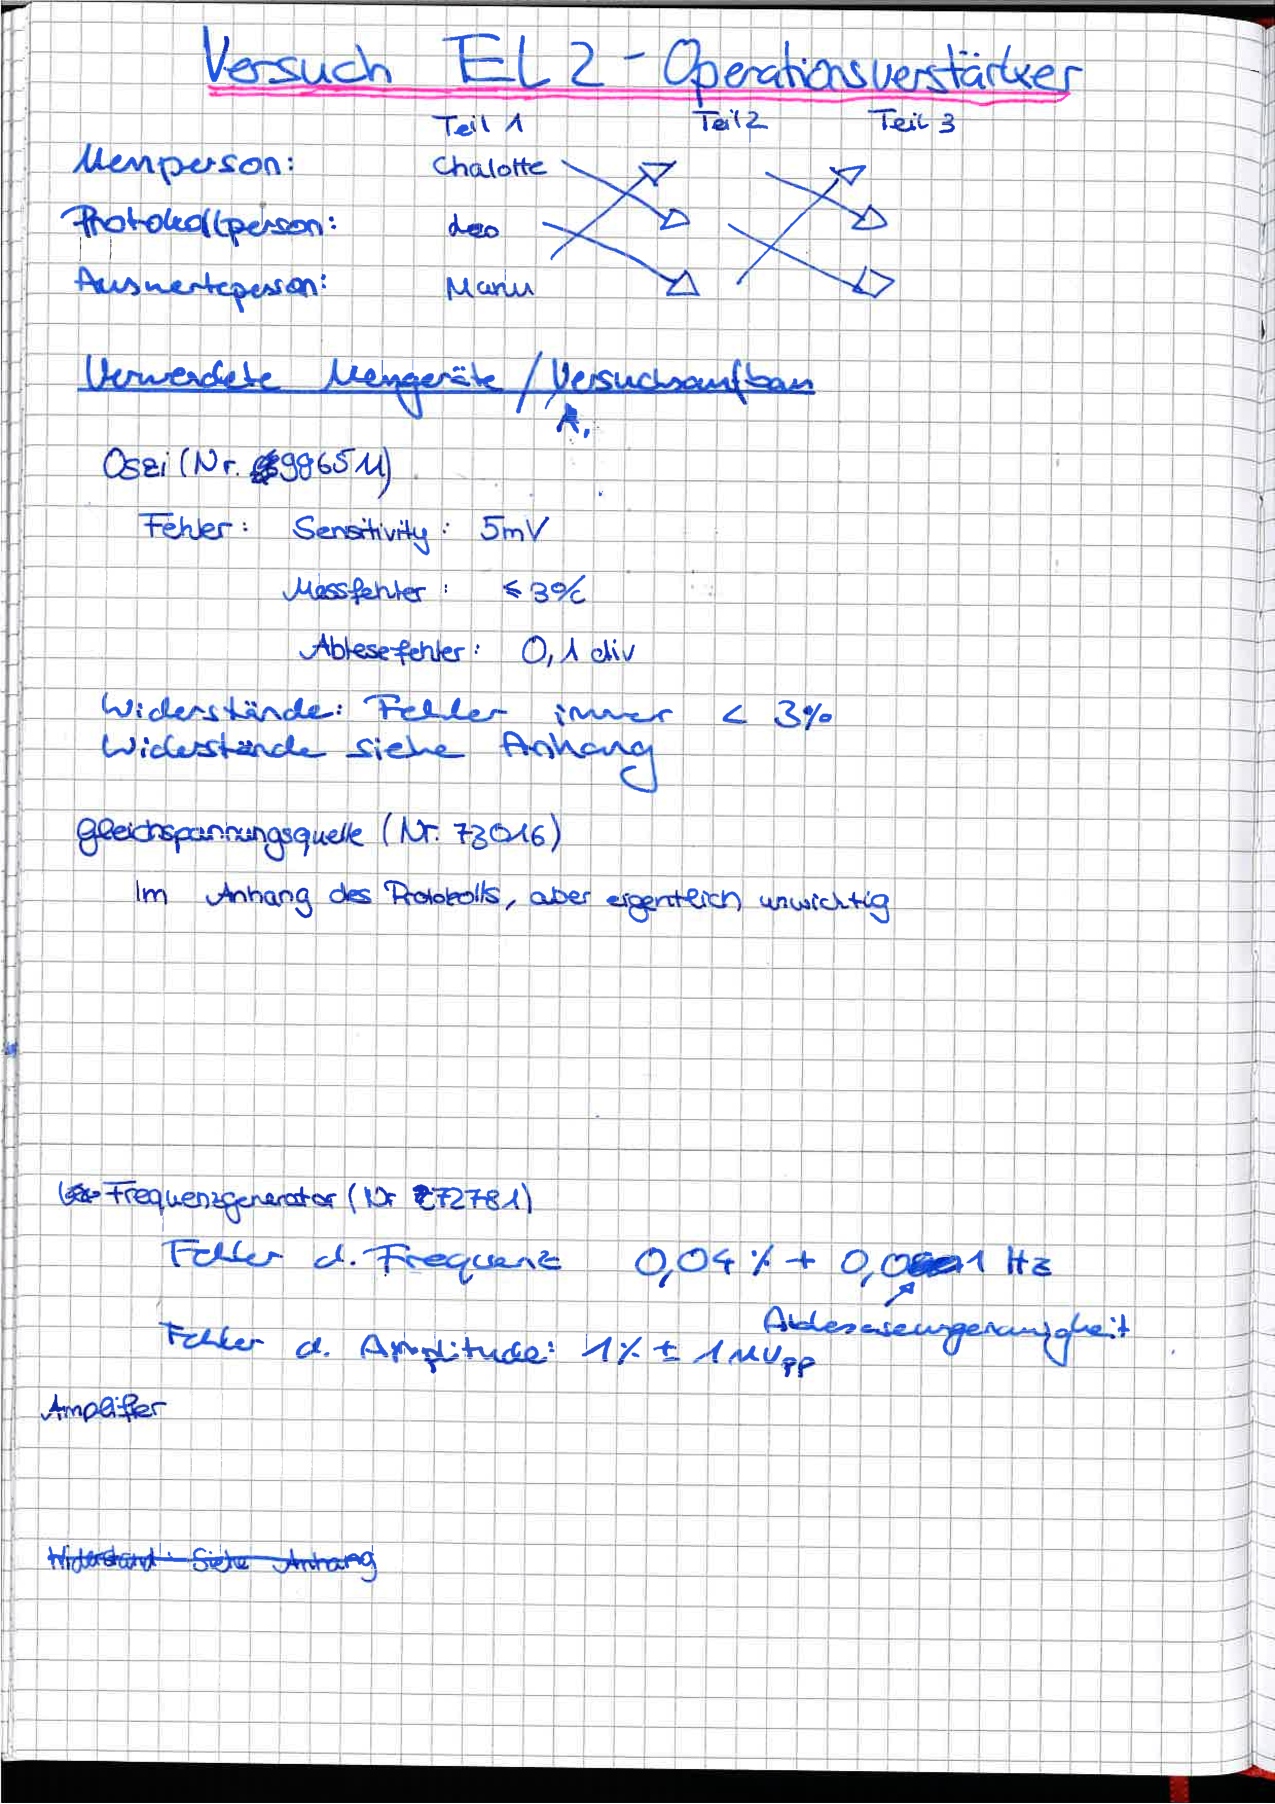
\includepdf[pages = -, landscape = false, nup = 1x1, scale = \skalierung , pagecommand={}]{30-ProtokollEL2.pdf}

%\section*{Steckbretter}
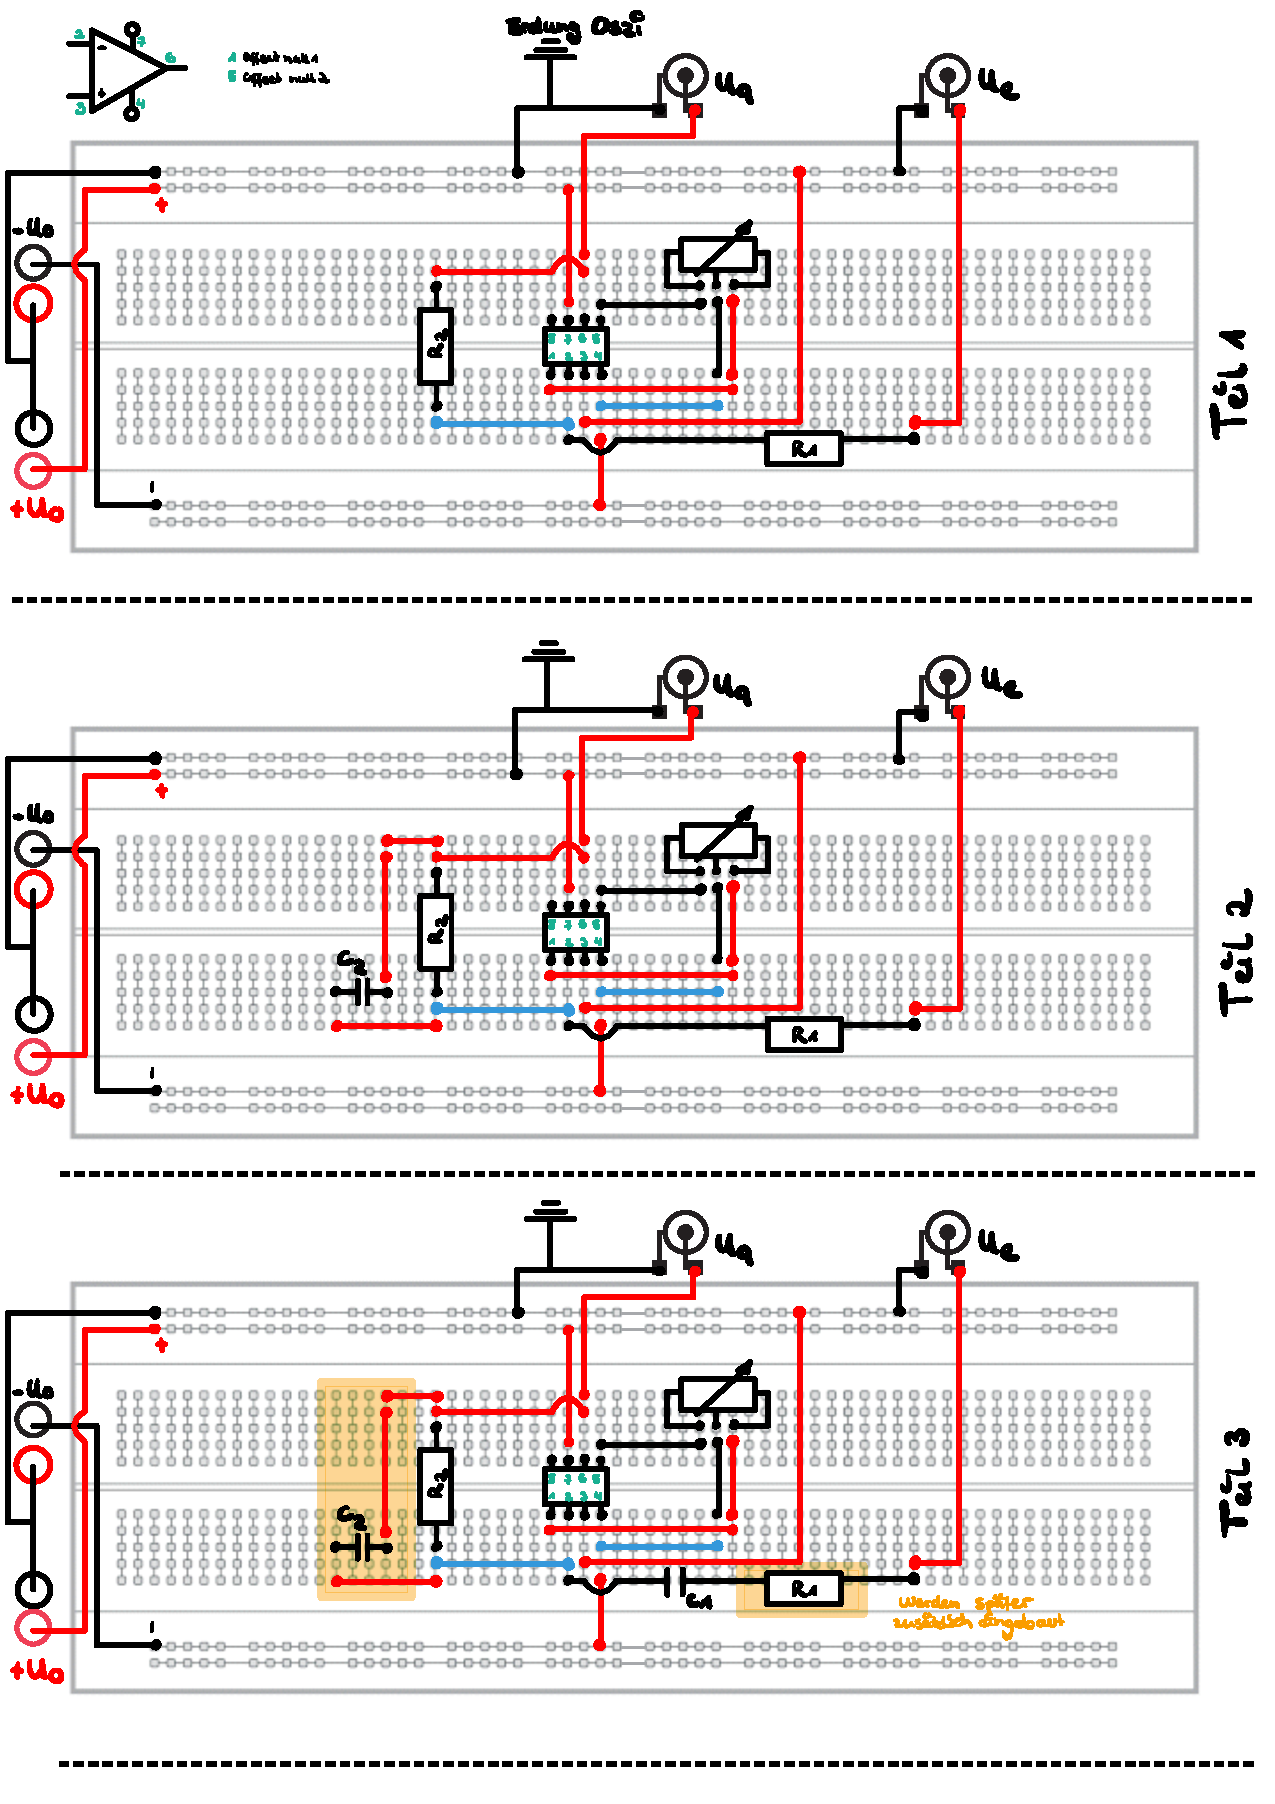
\includepdf[pages = 1, landscape = false, nup = 1x1, scale = \skalierung , pagecommand={}]{30-SteckbretterEL2.pdf}


    % 4.Kapitel Versuchsauswertung
    % Manuel Lippert - Paul Schwanitz
% Physikalisches Praktikum

% 4.Kapitel Versuchsauswertung

\chapter{Auswertung und Diskussion}
\label{chap:versuchsauswertung}

% Text

% Input der Teilauswertung je nach Produktion der Nebendateien ohne Ordner
%Matteo Kumar - Leonhard Schatt
% Fortgeschrittenes Physikalisches Praktikum

% Teilauswertung X

\section{Teilauswertung X}

% etc.

    % 5.Kapitel Fazit
    % 5. Fazit

\chapter{Fazit}
\label{chap:fazit}


% Text

    % Matteo Kumar - Leonard Schatt
% Physikalisches Praktikum

% Anhang

\appendix

% Text

% Charlotte Geiger - Manuel Lippert - Leonard Schatt
% Physikalisches Praktikum

% Anhang A

\chapter{Append A}
\label{chap:anhangA}

\section{Teilanhang X}


    % Literatur
    \bibliographystyle{Auswertung.bst}
    %\nocite{*}
    \bibliography{Auswertung.bib}

\end{document}